\chapter{Methodology} \label{cp:methodology}

\section{Apparatus} \label{sec:apparatus}
A Schlieren Imaging System is set up to view flow through a converging-diverging nozzle in the test section of the supersonic wind tunnel. The wind tunnel is seen in \autoref{fig:supersonic_wind_tunnel} with the nozzle shown in \autoref{fig:de_laval_nozzle}. A light source is reflected off a concave mirror which passes the light through the test section. Then, the light is reflected by another concave mirror towards a whiteboard after some of the focused light is blocked by a razor's edge. A camera is used to capture the projection on the whiteboard (see \autoref{fig:schlieren_projection}) which is connected to a delay generator to match the images with pressure data from taps in the nozzle. The camera images and pressure transducer data are collected using data acquisition software on a computer. 

\begin{figure}[htpb]
    \centering
    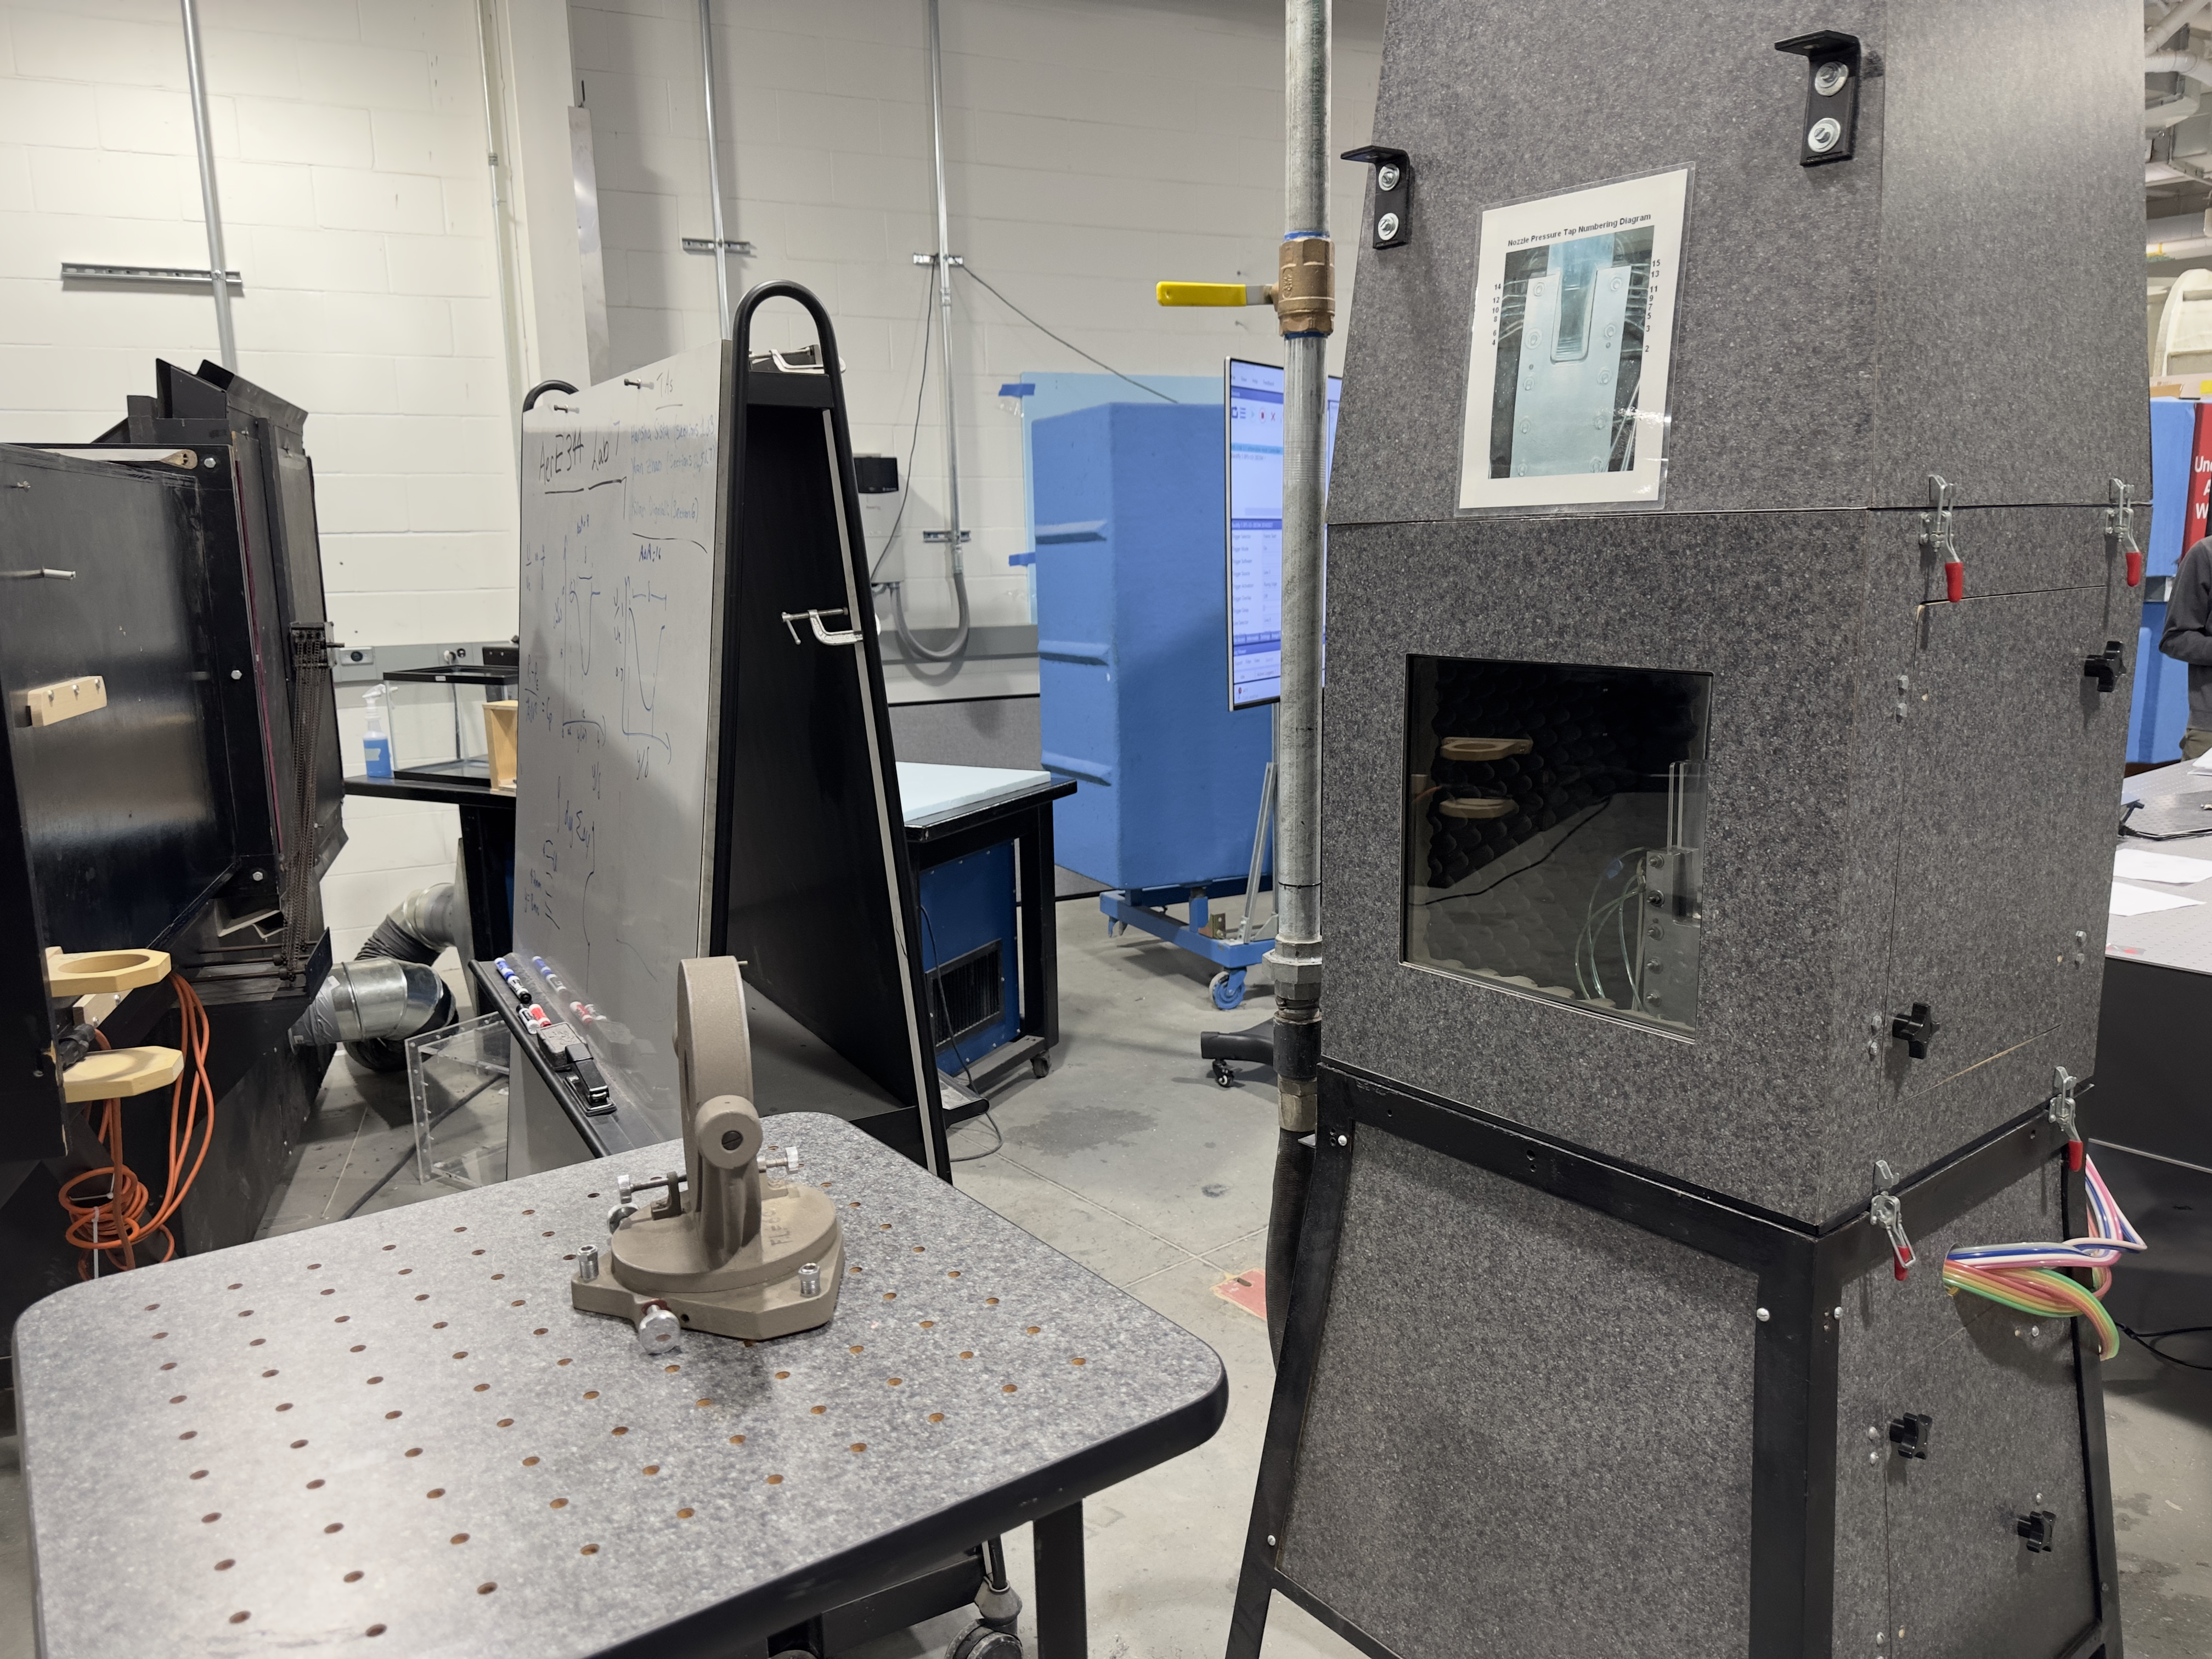
\includegraphics[width=0.75\linewidth]{Figures/back_of_supersonic_wind_tunnel.jpeg}
    \caption{The supersonic wind tunnel.}
    \label{fig:supersonic_wind_tunnel}
\end{figure}

\begin{figure}[htpb]
    \centering
    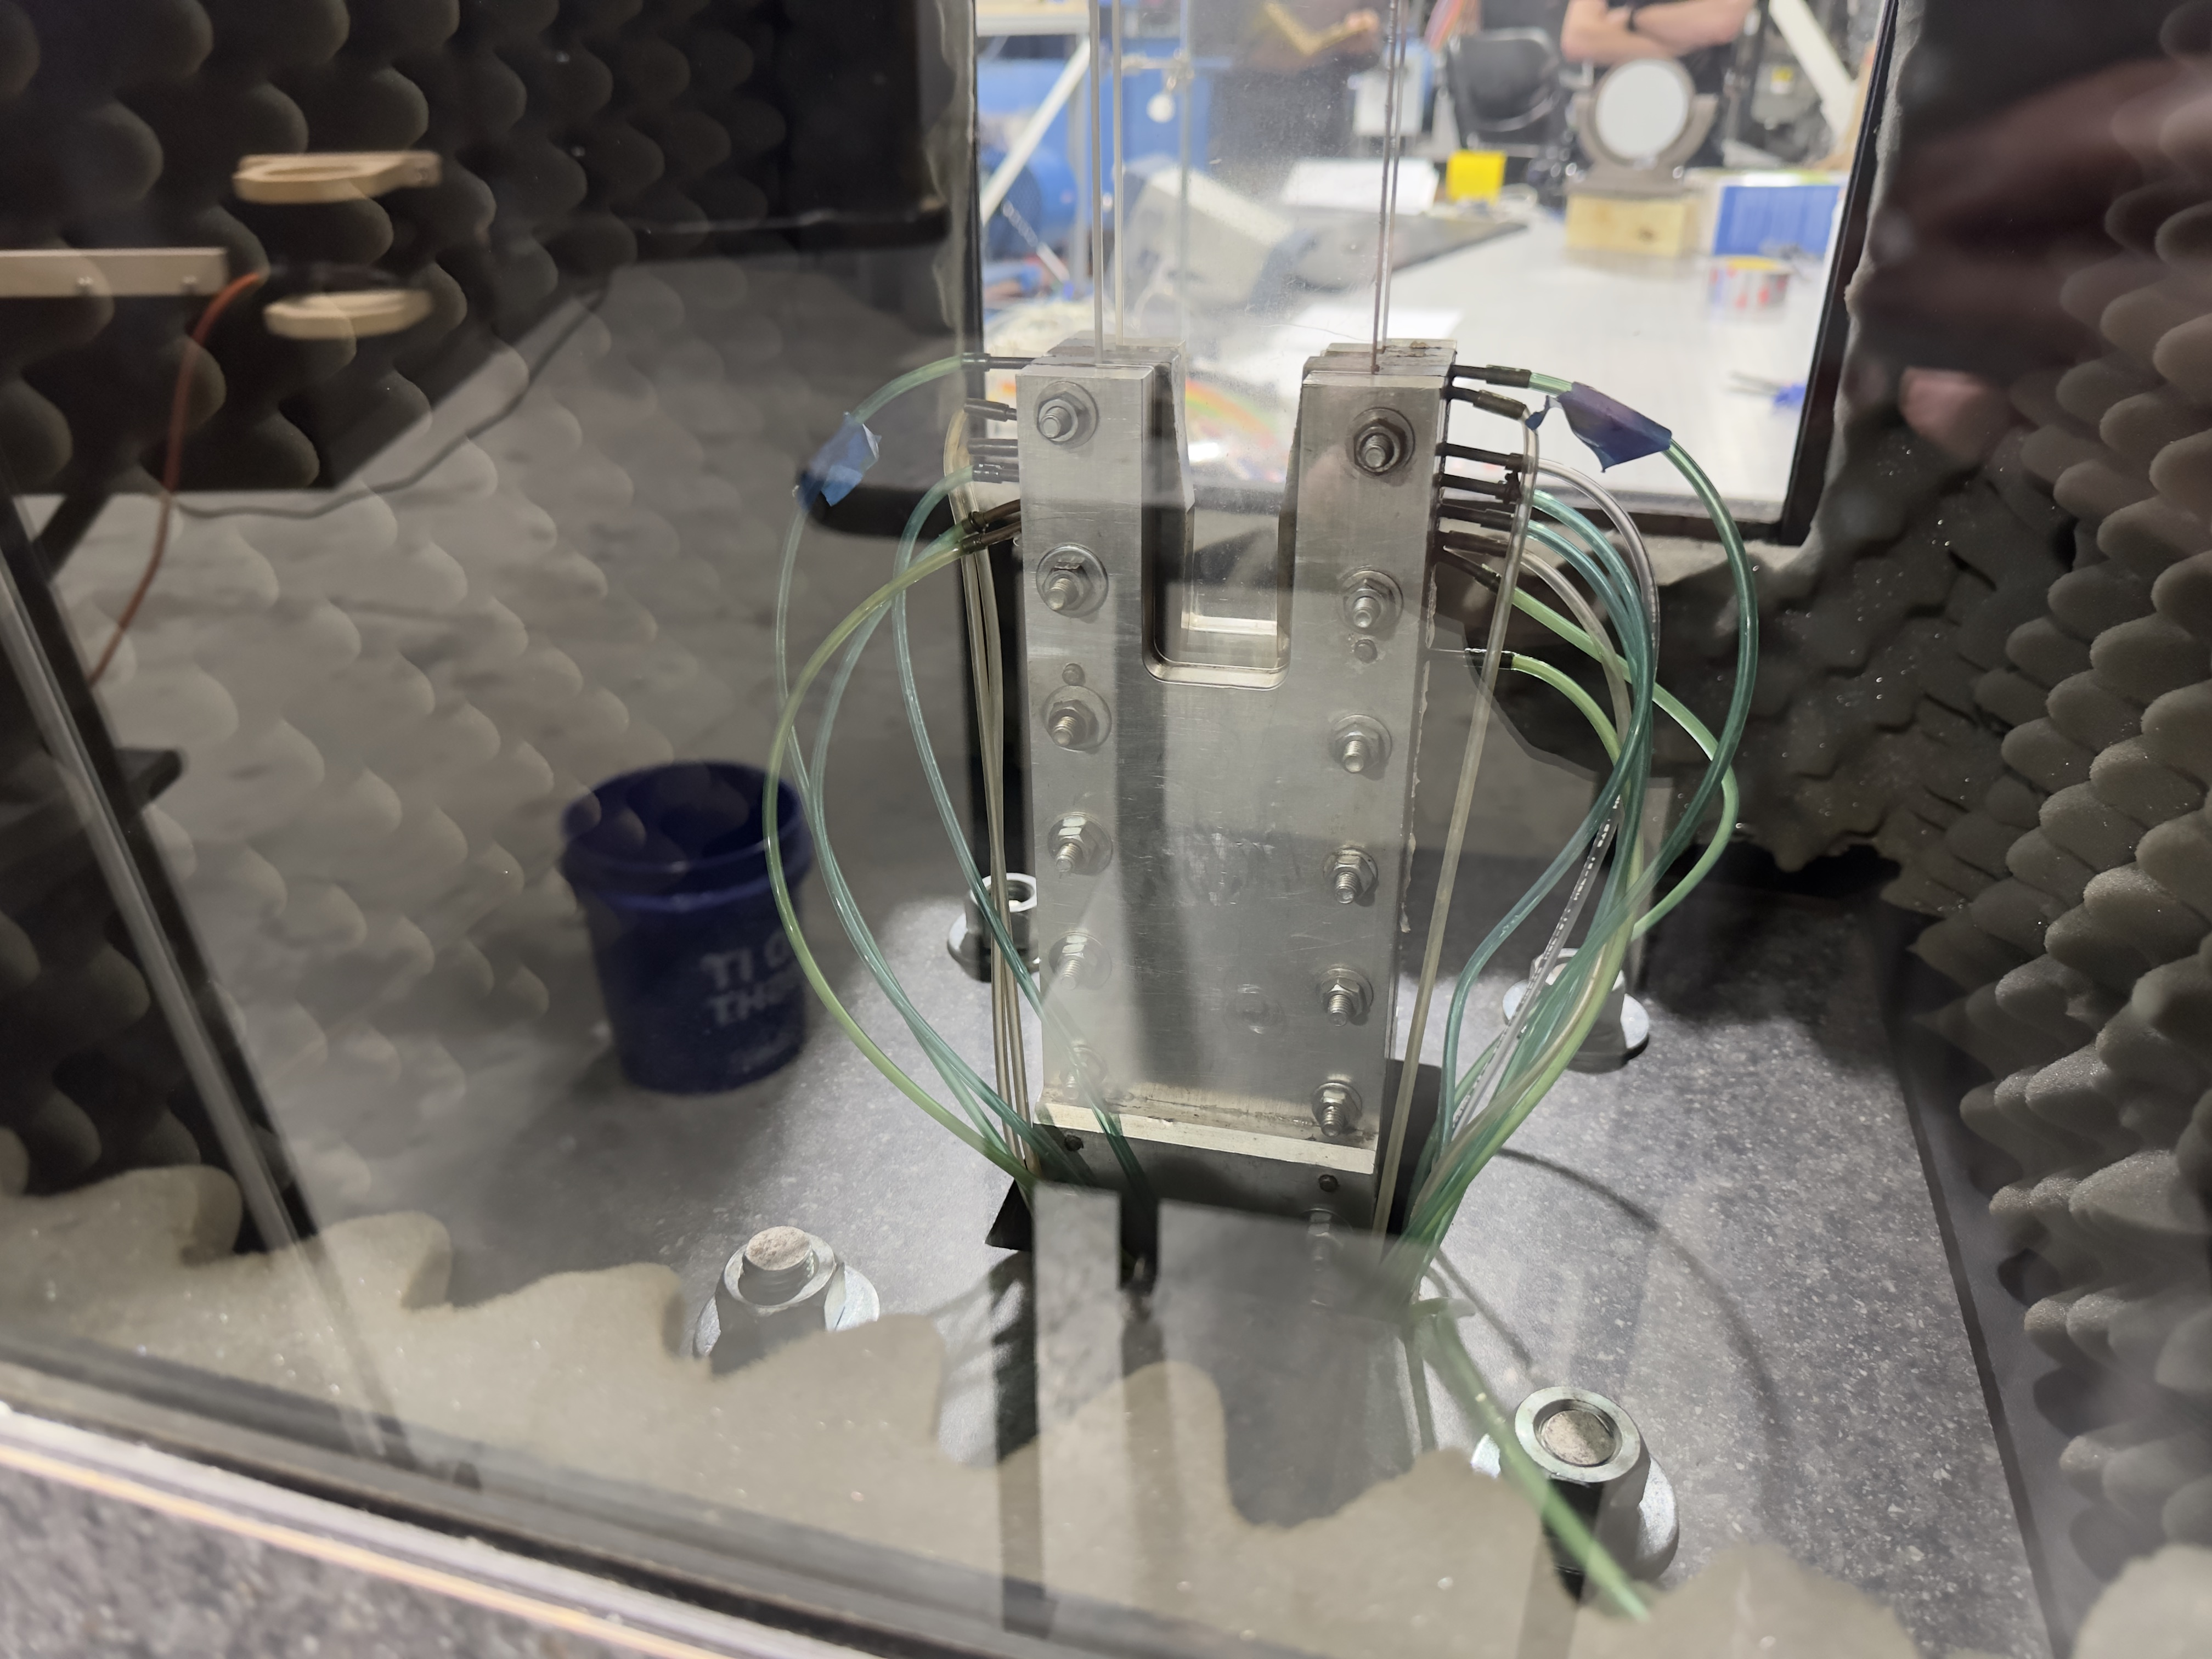
\includegraphics[width=0.75\linewidth]{Figures/de_laval_nozzle.jpeg}
    \caption[The de Laval nozzle in the supersonic wind tunnel.]{The de Laval nozzle in the supersonic wind tunnel. The pressure taps are connected to a pressure transducer which is further connected to the data acquisition computer.}
    \label{fig:de_laval_nozzle}
\end{figure}

\begin{figure}[htpb]
    \centering
    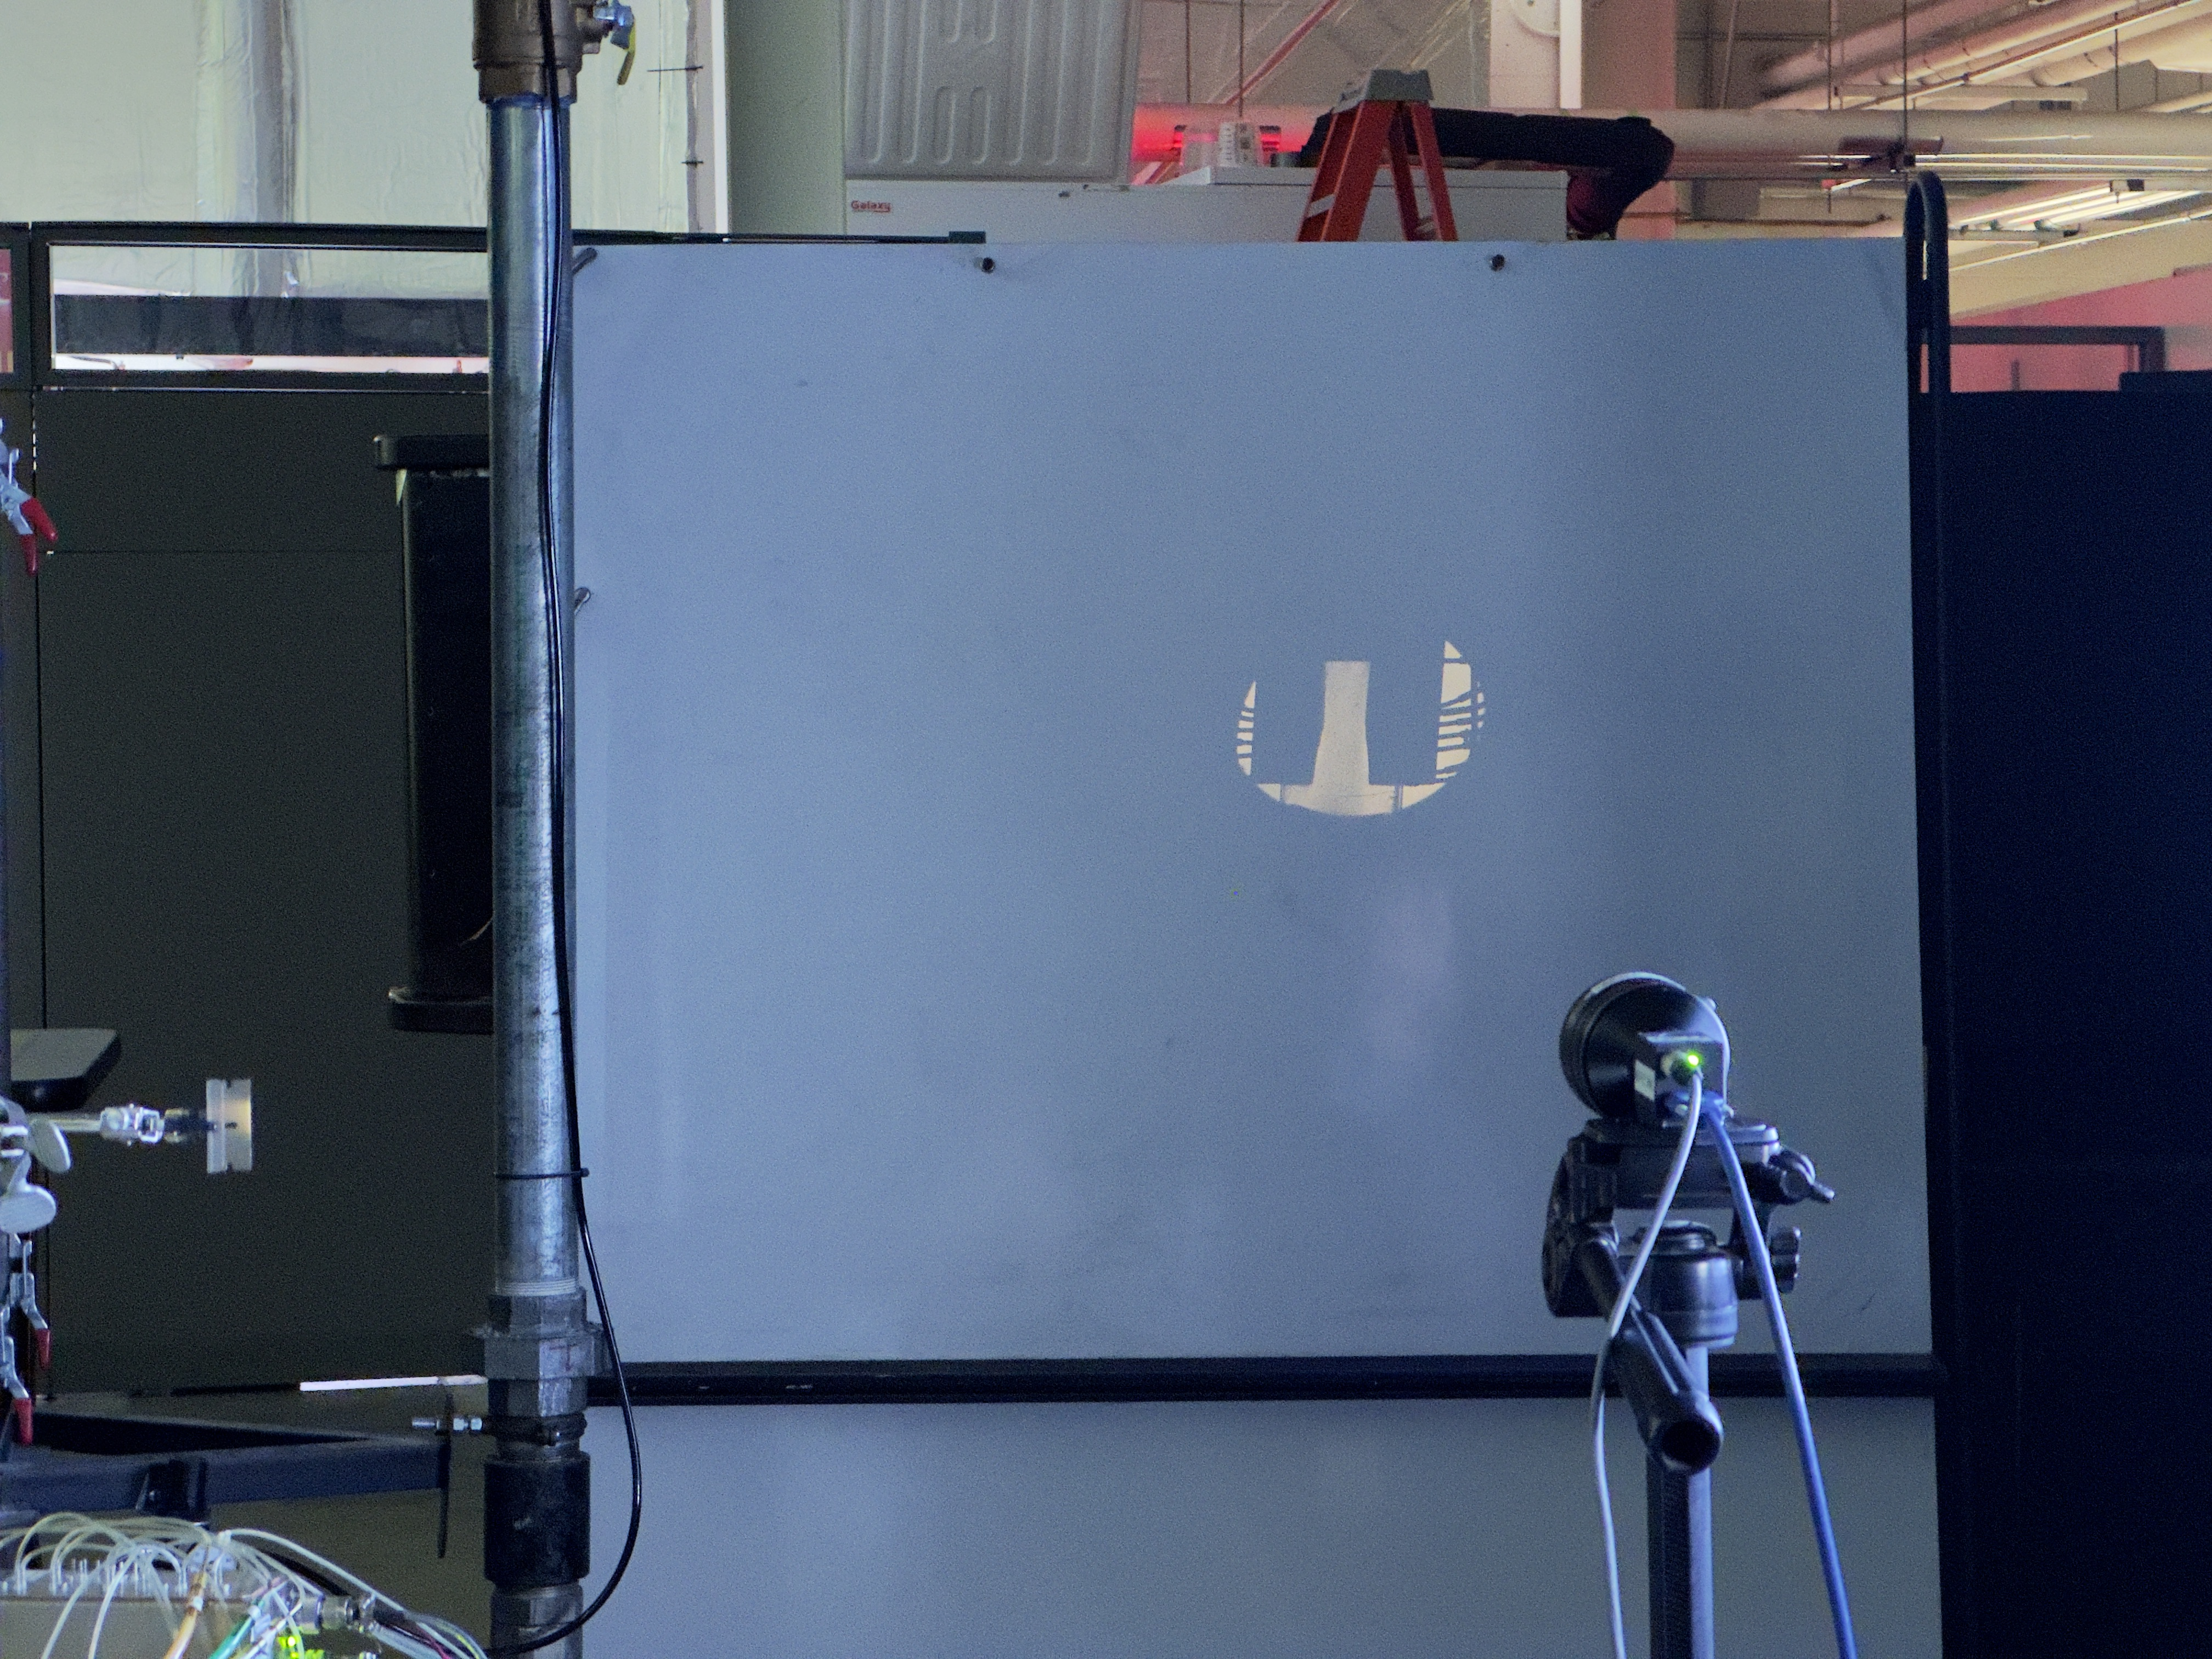
\includegraphics[width=0.75\linewidth]{Figures/schlieren_nozzle.jpeg}
    \caption[A Schlieren projection of the flow moving through the de Laval nozzle being projected onto a white board.]{A Schlieren projection of the flow moving through the de Laval nozzle being projected onto a white board. The camera takes close-up, high-contrast images of the projection.}
    \label{fig:schlieren_projection}
\end{figure}

\section{Procedure} \label{sec:procedure}

\begin{enumerate}
    \item Pressurize the air tank connected to the supersonic wind tunnel.
    \item Set up the imaging system as described in \autoref{sec:apparatus}.
    \item Start recording data using the data collection software and open the valve to release the air into the wind tunnel.
    \item When the tank is empty, close the valve.
\end{enumerate}

\section{Derivations} \label{sec:derivations}

There are a number of calculations that must be performed on the measured data before it can be compared to the theoretical calculations. Namely, we must transform a series of pressure tap measurements that are measuring static gauge pressure into a distribution of pressure and total pressure. The details of these calculations for the measured and theoretical scenarios can be found in \autoref{sec:measured_calculations} and \autoref{sec:theoretical_calculations}, respectively.

For the sake of comparison, we choose picture or data point number \num{168} (zero-indexed) for our state with a normal shock in the divergent section of nozzle. The image from this data point is shown in \autoref{fig:schlieren_overlay} with the schematic of the de Laval nozzle overlaid. The data shows a significant drop in static pressure between pressure taps \num{10} and \num{11}, but from the image, it appears that the normal shock is in between pressure tap \num{11} and \num{12}.

Because of the boundary layer conditions, the normal shock does not span straight across the nozzle, and the slight curvature of the shock near the edges of the nozzle may explain why the shock appears to be between taps \num{11} and \num{12} but the pressure drop occurs between taps \num{10} and \num{11}. For the sake of analysis, we chose to assume the normal shock occured between pressure taps \num{10} and \num{11} with the pressure at tap \num{10} and \num{11} denoted \gls{P_1} and \gls{P_2}, respectively.

\begin{figure}[htpb]
    \centering
    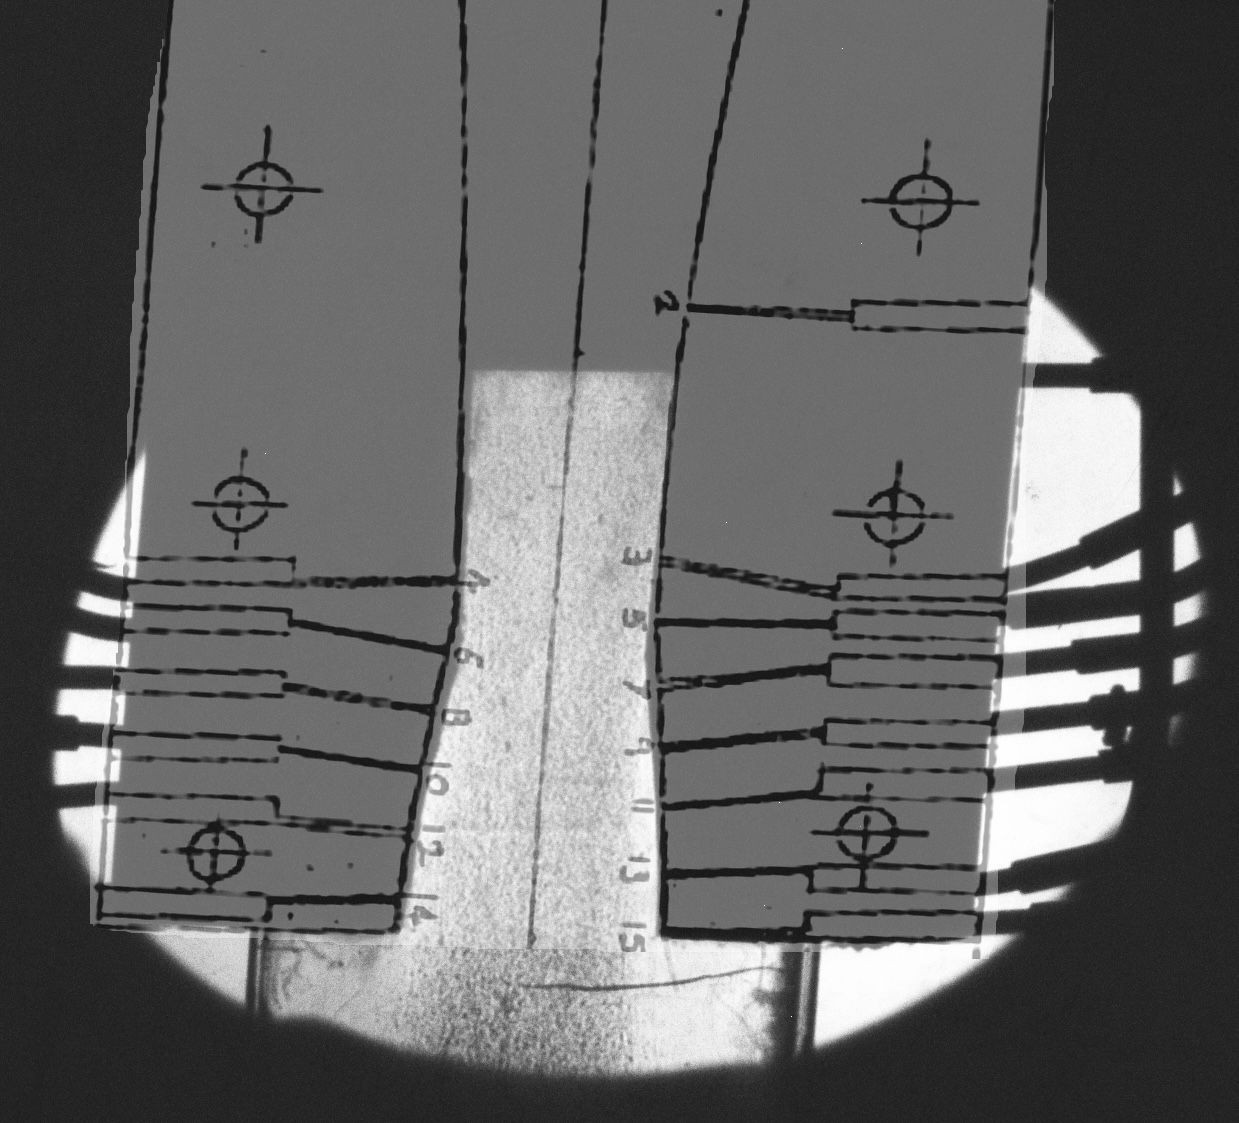
\includegraphics[width=\linewidth]{Figures/Nozzle Overlay with Shock.jpg}
    \caption[An overlay of the de Laval nozzle schematic and an image of the nozzle when a normal shock is present.]{An overlay of the de Laval nozzle schematic and a Schlieren image capture of the de Laval nozzle when the shock is inside the divergent section of the nozzle.}
    \label{fig:schlieren_overlay}
\end{figure}

\subsection{Measured Calculations} \label{sec:measured_calculations}


\subsection{Theoretical Calculations} \label{sec:theoretical_calculations}
